\documentclass[../main.tex]{subfiles}

\begin{document}
Two main problems of calculus are
\begin{enumerate}
  \item Derivative. Find the rate of change of $f$.
  \item Integral. Find the area under a given curve.
\end{enumerate}
Both are based on the concept of limit.

We say $\lim_{x \to a} f(x) = L$ to mean $f(x)$ is ``close enough'' to $L$ when $x$ is ``close enough'' to \emph{but not equal to} $a$.

\begin{example}
  $\lim_{x \to a} x = a$. $x$ is close enough to $a$ when $x$ is close enough to $a$.
\end{example}

\begin{example}
  $\lim_{x \to a} c = c$ if $c$ is a constant.
\end{example}

\begin{example}
  \[
    g(x) =
    \begin{cases}
      x, &\text{ if } x\neq 2\\
      1, &\text{ if } x = 2\\
    \end{cases}
  \]
  $\lim_{x \to 2} g(x) = \lim_{x \to 2} x = 2$ although $g(2) = 1$.
\end{example}

\subsection*{One-sided limits}
If $f(x)$ is close to $L$ when $x<a$ is close enough to $a$ then we say
\[
  \lim_{x \to a^{-}} f(x) = L
\]
This is called the \emph{left limit} of $f$ at $x=a$.

Similarly we can define the right limit.

\begin{example}
  \[
  f(x) =
  \begin{cases}
    -1 & \text{for $x<0$}\\ 0 & \text{for $x=0$}\\ 1 & \text{for $x>0$}
  \end{cases}
  \]
  \begin{figure}[ht]
    
\begin{picture} (180.000000,83.371429)(0,0)
\put(0.0, 0.0){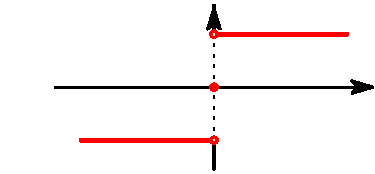
\includegraphics{figures/03signOFx.pdf}}
    \put(128.14,  75.11){\sffamily\itshape $y=f(x)$}
    \put( 99.71,  65.11){\sffamily\itshape \makebox[0pt][r]{$1$}}
    \put(104.71,  14.26){\sffamily\itshape \makebox[0pt][l]{$-1$}}
\end{picture}

    \caption{The sign function.}
  \end{figure}

  \[
  \lim_{x\to 0} f(x) \text{ does not exist.}
  \]

  In this example the one-sided limits do exist, namely,
  \[
  \lim_{x\searrow0}f(x) = 1 \text{ and } \lim_{_x\nearrow0}f(x) = -1.
  \]
\end{example}

\begin{example} Evaluate the expressions by referencing the plot in Figure~\ref{plot:piecewise-exercise}.
\begin{figure}
\begin{tikzpicture}
  \begin{axis}[
            domain=-4:6, xmin=-4, xmax=6, ymin=-3,ymax=10,
            unit vector ratio*=1 1 1,
            axis lines =middle, xlabel=$x$, ylabel=$y$,
            every axis y label/.style={at=(current axis.above origin),anchor=south},
            every axis x label/.style={at=(current axis.right of origin),anchor=west},
            xtick={-4,...,6}, ytick={-3,...,10},
            xticklabels={-4,,-2,,0,,2,,4,,6}, yticklabels={,-2,,0,,2,,4,,6,,8,,10},
            grid=major,
            grid style={dashed, gridColor},
          ]
    \addplot [very thick, penColor, smooth, domain=(-4:-2)] {6};
    \addplot [very thick, penColor, smooth, domain=(-2:0)] {x^2-2};
          \addplot [very thick, penColor, smooth, domain=(0:2)] {(x-1)^3+3*(x-1)+3};
          \addplot [very thick, penColor, smooth, domain=(2:6)] {(x-4)^3+8};
          \addplot[color=penColor,fill=background,only marks,mark=*] coordinates{(-2,6)};  %% open hole
          \addplot[color=penColor,fill=background,only marks,mark=*] coordinates{(-2,2)};  %% open hole
          \addplot[color=penColor,fill=background,only marks,mark=*] coordinates{(0,-2)};  %% open hole
          \addplot[color=penColor,fill=background,only marks,mark=*] coordinates{(0,-1)};  %% open hole
          \addplot[color=penColor,fill=background,only marks,mark=*] coordinates{(2,0)};  %% open hole
          \addplot[color=penColor,fill=penColor,only marks,mark=*] coordinates{(-2,8)};  %% closed hole
          \addplot[color=penColor,fill=penColor,only marks,mark=*] coordinates{(0,-1.5)};  %% closed hole
          \addplot[color=penColor,fill=penColor,only marks,mark=*] coordinates{(2,7)};  %% closed hole
        \end{axis}
\end{tikzpicture}
\caption{A plot of $f(x)$, a piecewise defined function.}
\label{plot:piecewise-exercise}
\end{figure}
\begin{enumerate}
\begin{multicols}{3}
\item $\lim_{x\to 4} f(x)$
\item $\lim_{x\to -3} f(x)$
\item $\lim_{x\to 0} f(x)$
\item $\lim_{x\to 0-} f(x)$
\item $\lim_{x\to 0+} f(x)$
\item $f(-2)$
\item $\lim_{x\to 2-} f(x)$
\item $\lim_{x\to -2-} f(x)$
\item $\lim_{x\to 0} f(x+1)$
\item $f(0)$
\item $\lim_{x\to 1-} f(x-4)$
\item $\lim_{x\to 0+} f(x-2)$
\end{multicols}
\end{enumerate}

(a) $8$, (b) $6$, (c) DNE,
(d) $-2$, (e) $-1$, (f) $8$,
(g) $7$, (h) $6$, (i) $3$,
(j) $-3/2$, (k) $6$, (l) $2$
\end{example}

\end{document}